\chapter{Object Detection} \label{sec:det}
This chapter will present the algorithm used for the object detection. First the conditions imposed by the vehicle and the Carolo-Cup regulations are listed. Next the algorithms currently used for obstacle-, sign-, pedestrian- and slope-detection and their drawbacks are presented. 
Next related work is presented, thereafter the algorithm that provides the basis for the proposed algorithm is presented. Lastly the changes to the algorithm that improve the performance on dense stereo point clouds are presented.

\section{Conditions Imposed by the Carolo-Cup Regulations}

\subsection{Carolo-Cup} \label{sec:det:ccr}
The Carolo-Cup is an international student competition in which students have to develop and build an automated 1:10 scaled model car.
The competition is held in Braunschweig, annually since 2008. It consists of three disciplines: the presentation in which the team has to explain their concept in front of a jury, free drive which requires the vehicle to drive as many meters as possible on a simple track and obstacle course which consists of a track with intersections, pedestrian crossings, speed limits, obstacles and pedestrian islands in abstracted form.

The possible situations and objects are defined by the Carolo-Cup regulations \cite{Carolo-CupRegelwerk}. 
In the following passage the aspects of the regulations which are relevant for this thesis are explained in more detail.

\subsubsection{Obstacles}
Obstacles, which represent other vehicles, can be present anywhere on the track. 
If they are on the same side of the road as the vehicle they need to be passed. If they are waiting at intersections the right of way has to be observed.

Obstacles are white boxes with a width of 100 to 400mm, a height of 100 to 240mm and a minimal length of 100mm. They are either static or dynamic, if they are dynamic they move at a speed of 0.6m/s.

\subsubsection{Pedestrians}
Pedestrians can wait on the side of a track, if they are next to a crosswalk the vehicle has to let them pass.

Pedestrians are represented by white boxes with a width of 100mm and a height of 150mm. Solely by their size or shape, pedestrians can not be differentiated from obstacles, to differentiate them a black stick figure is visible on the side of the box facing the vehicle.

\subsubsection{Signs}
Traffic signs are placed to the right of the track and mark speed limits, intersections, crosswalks, expressways, sharp turns, barred areas, no passing zones and slopes.
They are placed at a height of 150mm. Their width and height is between 100mm and 150mm depending on the type of the sign.

\subsubsection{Slopes} \label{sec:det:ramp}
Parts of the track can consist of slopes of up to 10\%. Each of the features that can occur on the track can occur on the slope as well. Usually a single ramp, that is an incline, followed by a flat part and a decline exists on a track.

\subsection{Vehicle}
All vehicles are based on a 1:10 \ac{rc}-chassis, for the computations an Intel \ac{nuc} Skull Canyon is used. The main sensors are a colour camera and depth camera.

\subsubsection{Depth Camera}
The depth camera used in the vehicle is an \ac{d435}. It uses a stereo camera system and an infrared projector for active stereo \cite{D435}. 
The depth camera has a resolution of up to 1280x720 and can acquire up to 90 \ac{fps} at a lower resolution. 
At the full resolution the camera provides a maximum frame rate of 30 \ac{fps}.
Additionally the \ac{d435} provides a colour image, due to the poor performance of the sensor the image is not usable if the vehicle is moving.

The vehicle is equipped with a single \ac{d435} pointed forward. The maximum range of the camera is approximately ten meters. 

\subsubsection{Software Environment}
The software on the vehicle is written in C++ and using \ac{adtf} as framework for communication and scheduling.
To guarantee a fast response of the vehicle to an input all software running on the vehicle needs to meet certain soft real-time criteria, this means in particular, that all algorithms need to run in a fixed time most of the time. For the perception layer of the software the maximum runtime of every perception is bound to the sampling period of the respective sensor.

\subsubsection{Maximum Required Detection Distance}
The vehicle drives with a maximum speed of $5\si{\m\s^{-1}}$ during the free drive, the maximum braking acceleration possible is $5\si{\m\s^{-2}}$ . 
The processing delay of the complete software of the vehicle can be calculated as the sum of the individual delays of the components: the \ac{d435} introduces a delay as a result of the limited frame rate. All parts of the vehicle software, that are the object detection, the tracking, the planning, the trajectory planning and the controller are estimated by the maximum time each module is allowed to run, this time is given by the frequency at which the respective module gets called. 
The latency of the hardware is defined by the frequency at which messages get sent to the motor controller.

\begin{eqnarray}
    t_\text{processing} &\leq& t_\text{D435} + t_\text{detection} + t_\text{tracking} \\  
                        &+& t_\text{planning} + t_\text{trajectory} + t_\text{controller} + t_\text{hardware} \nonumber \\
                      &=& 33 \si{\ms} + 33 \si{\ms} + 5 \si{\ms} + 5 \si{\ms} + 5\si{\ms} + 5\si{\ms} + 10 \si{\ms} = 96 \si{\ms} \nonumber
\end{eqnarray}

The maximum distance for the vehicle to stop can be calculated as the sum of the distance the vehicle drives during the processing time and the braking distance:

\begin{eqnarray}
    s &\leq& v_\text{max} \cdot t_\text{processing} + \frac{1}{2} \frac{v_\text{max}^2}{a_\text{braking}} \\
    &=& 5 \si{\m \per \s} \cdot 0.096 \si{\s} 
        + \frac{1}{2} \frac{{(5\si{\m \per \s})}^2}{5 \si{\m \per \square \s}} \nonumber \\
    &=& 0.48 \si{\m} + 2.5 \si{\m} = 2.98 \si{\m} \nonumber
\end{eqnarray}

Thus it is for the detection sufficient to detect objects at a distance of up to three meters. 

\section{Current State}
At the moment the obstacles and the signs are detected by two different detectors. As a result obstacles are often detected as signs and vice versa, and thus require additional filtering. Additionally both algorithms yield poor results when the ground is not at a constant height.

\subsection{Obstacle Detection} \label{sec:det:obstDet}
The obstacle detection was initially developed as part of a Bachelor's Thesis \cite{marceldebout2012}.
For the detection all points at a fixed height relative to the camera are extracted from the point cloud, this height is $0.1\si{\m}$ above the ground as this is the minimum size of obstacles. This reduces the detection to a two dimensional problem and decreases the number of points.
Figure \ref{fig:det:dbtopdown} shows the points (in red) extracted from a point cloud. The vehicle is visualized by the blue circle on the left side of the figure.

For the detection all points on this plane are clustered using the DBGridScan-Algorithm \cite{danielmeisner2016}. 
In the last step a bounding box is estimated, for the estimation the algorithm differentiates between so-called I- and L-Shapes. 
I-Shapes are objects with only one side visible in the point cloud, L-Shapes objects of which two sides can be seen in the point cloud.
For I-Shapes the bounding box is assumed to be square, the length of all sides is estimated to be the same as the length of the visible side. 
For L-Shapes the bounding box is assumed to be a parallelogram, for this the fourth, not visible, corner is calculated based on the three visible corners.

\begin{figure}[h!]
    \centering
    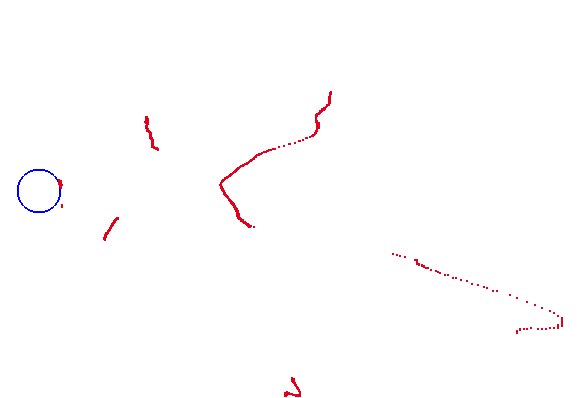
\includegraphics[width=\textwidth]{../Material/depth_slice.png}
    \caption{Top down view of the points used for the DBGridScan-Algorithm}
    \label{fig:det:dbtopdown}
\end{figure}

Most steps of the detection are done in two dimensions, assuming that the ground is at a constant height. 
Due to the introduction of slopes (see \ref{sec:det:ramp}) in 2017 this does not hold anymore. 
As a result the algorithm detects these slopes as obstacles. 
Furthermore it does not detect obstacles if these obstacles are at a different height than expected due to a slope.

To avoid false positives the detection is done at three heights independent of each other. 
Then it is checked for every obstacle if it is present on all three heights, for slopes this is not the case. 
This solves the problems related to false positives but does not help with the true negatives: obstacles which do not get detected as they are at a different height than expected due to a slope.

\subsection{Sign Detection}
As the computer on the vehicle has only a limited amount of computational resources the detection can not be done with state of the art detectors such as R-CNN \cite{rcnn}, Single-Shot-Detector \cite{ssd} or YOLO \cite{yolo}. The detection of the traffic signs is done with the depth data of the \ac{d435}. The detection estimates a bounding box for the signs, this bounding box gets mapped into the image of the main camera and an image is extracted. This image is then classified using a \ac{cnn}.

Multiple lines are scanned in the depth image to find large differences in distance which resemble an edge.
With these edges bounding boxes for sign candidates are extracted, these candidates are filtered based on their size, position and form. The \ac{cnn} then determines if the candidate is a valid sign and the type of the sign if it is one.

\begin{figure}[h]
    \centering
    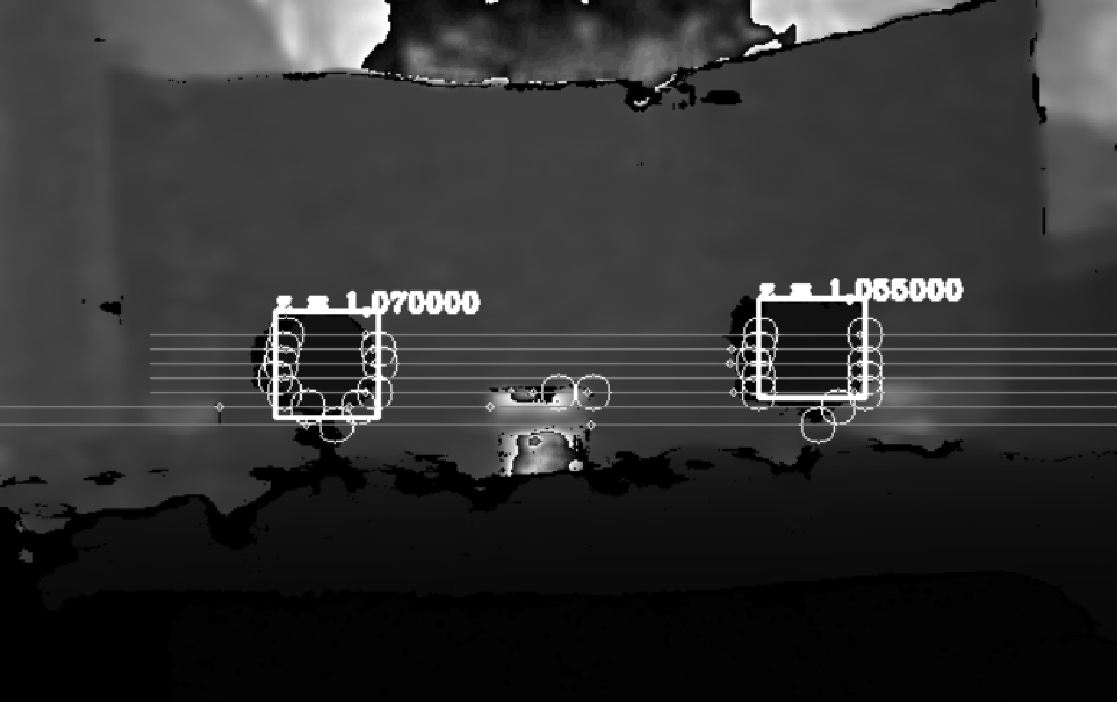
\includegraphics[width=\textwidth]{../Material/sign_depth_detection.png}
    \caption{Lines scanned by the sign detection}
    \label{fig:det:signScan}
\end{figure}

Figure \ref{fig:det:signScan} shows a disparity map of the camera. The lines along which the image is scanned, detected edges along these lines and filtered candidates are highlighted.

Similar to the obstacle detection the sign detection has difficulties with signs which are not on the expected height. Therefore some signs which are located on slopes do not get detected.

\subsection{Pedestrian Detection}
The detection of pedestrians is done twofold: as pedestrians are valid obstacles they get detected by the obstacle detection. 
This is done primarily to detect moving pedestrians at crosswalks. 
As there are no obstacles on crosswalks the contextual information can be used to differentiate between obstacles and pedestrians. 

Due to the small field of view of the \ac{d435}, pedestrians standing next to the road can not be detected by the obstacle detection. 
The detection of these pedestrians is done with a simple blob detector in the camera image if the vehicle is at a crosswalk.

\subsection{Slope Detection}
At the moment the slope of a ramp can not be detected by the vehicle. 
At the start of every slope there is a sign which signals the oncoming slope, if this sign is detected the vehicle decreases its speed.
Due to the problems listed above the sign is often not detected. Additionally there are problems with the lane and road markings detection on the ramp, this is because the complete image is warped on the ramp and as a result the extrinsic calibration is wrong and distances are estimated wrongly.

\section{Related Work}
In recent years many algorithms for object detection in point clouds have been proposed. 
Most of them do an end-to-end detection using a large \ac{cnn} \cite{Yin17} \cite{Bin19} \cite{Mar18} \cite{Li16}, for these networks the data is usually represented by voxels, which are pixels in the three dimensional space, or by a two dimensional map-like representation.
Due to the limitations in computational performance on the vehicle and the real time constraints it is not possible to use such a deep neural network for this task.
Faster algorithm rely on a separate detection and classification of the objects: first objects are detected in the point cloud, often using a clustering algorithm, then each cluster is classified.
For the clustering often an occupancy map is used, for most algorithms the classification is done with a learned classifier such as a support vector machine \cite{HivHWu10}, k-nearest neighbours \cite{YifeiTian18} or a \ac{cnn} \cite{AttBen17}.
Most of these algorithms are intended to be used with point clouds captured using a Lidar system.

For data acquired from stereo systems many algorithms use the disparity map for detection \cite{guindel18} \cite{qian16}. 
\cite{Wang19} discovered that the performance of object detection can be vastly improved by representing the data as a point cloud which correctly represents spatial relations, instead of disparity maps in which neighbouring pixels are not required to belong to the same object.

\section{Algorithm}
The following section introduces the proposed algorithm for object detection. 
The algorithm works in multiple steps: At first the algorithm decides for all points if it belongs to an object of interest, this step is referred to as segmentation. Next all points of interest are clustered to form objects. In the last step of the detection every cluster gets a type assigned. This is done by extracting a pseudo depth image for every cluster and classifying each depth image with a \ac{cnn}.

The algorithm is an improved version of \cite{AttBen17} to be used with point clouds generated from stereo systems instead of Lidar. 
It uses the point cloud as an input and detects the objects and determines the type of each object.
First the original algorithm is presented, then the improvements which enable the detection in stereo point clouds are presented.

Additionally to the improved algorithm of \cite{AttBen17} a bounding box is estimated for every cluster. Using points which do not belong to a cluster the ground is estimated by fitting a single plane.

\subsection{Segmentation}

\subsubsection{Grid}
All points of the point cloud are inserted into a grid. 
This is done by fitting a grid onto the $x$-$y$-plane, with the coordinate system defined like in section \ref{sec:theo:vehicleCoord}. 
The cells of the grid are equally sized. 
To reduce the number of points which need to be considered a region of interest for the grid is defined. 
For a point $\vec{p}$ given by $\vec{p} = {(x,y,z)}^\text{T}$, the region of interest is a function which defines for every
point if it is of interest:

\begin{equation}
    \text{ROI}\, (\vec{p}) = (0.2 \leq x \leq 3) \land (\abs{y} \leq 2) \land (-0.3 \leq z \leq 0.3)
\ \end{equation}

The cell a point belongs to is determined by projecting the point onto the $z=0$ plane. The point is then inserted into a set of points for the respective cell.

A cell $c$ is represented by a set of points:
\begin{equation}
    c = \{\vec{p}_1,\vec{p}_2, \ldots, \vec{p}_n \}\qquad \vec{p}_k \in \mathbb{R}^3,\ k \in \{1, \ldots, n\}
\end{equation}

\subsubsection{Classification}
The algorithm determines for every cell a type, the types are: Sparse, Low Foreground, High Foreground and Ground. 
The type Sparse is for cells which consist of few points, this is the case for cells which can not be seen by the sensor, either due to occlusion or due to the limited field of view.
The type Low Foreground is for all points which are part of an object such as cars and pedestrians, the type High Foreground is for points which belong to tall objects such as walls, the type Ground is for points which are part of the ground.

The type of each cell is calculated on the basis of the points in each cell. 
\cite{AttBen17} propose to determine the type of each cell based on the number of points, the minimum and the maximum height of all points in the cell. 

Cells with less than eight points are assigned the class Sparse. 
If the difference between the maximum and minimum height of the points in a cell is smaller than a predefined value the cell is labeled as ground.
A cell is classified as High Foreground if either the maximum height is larger than a threshold or the difference between the maximum and minimum height is larger than a threshold. 
All other cells are classified as Low Foreground.

\subsection{Clustering}
In the next step of the detection pipelines object candidates are extracted. This is done by clustering cells belonging to the class foreground. To improve the accuracy of the clustering it is done on a coarse and a fine level.

Two cells $c$ and $d$ belong to the same object if the coarse merging criterion $m_\text{Coarse}$ is fulfilled:
\begin{equation}
    m_\text{Coarse}\,  (c,d) = \abs{ \max_{{(x,y,z)}^\text{T} \in c}(z) - \max_{{(x,y,z)}^\text{T} \in d}(z) } < 0.05
\end{equation}
This yields clusters in which all cells have a similar maximum height. For the clustering the connected components labeling algorithm presented in section \ref{sec:theo:concomp} is used.

The coarse clustering limits the resolution of clusters to the size of a cell, to improve the accuracy clustering on a subcell level is performed. This is done by splitting every cell in a three times three grid, similar to the grid used for segmentation.

To be able to split objects which are close to each other \cite{AttBen14} proposed to do the second clustering step on the basis of the density of the cell. 
For this the ratio of the densities of two neighbouring cells is used. 
The criterion $m_\text{Fine}$, which indicates if two subcells $c$, $d$ belong to the same objects is:
\begin{equation}
    m_\text{Fine} = \frac{\max(\abs{c}, \abs{d})}{\min(\abs{c}, \abs{d})} < 10 
\end{equation}
This clustering step is only used to split objects which are close to each other, no existing clusters are merged.

\subsection{Extraction} \label{sec:det:originalExtraction}
After clustering each object needs to be classified. 
As small obstacles are of a similar size as signs it is not possible to classify the objects solely by size, the shape of the objects need to be taken into account as well. 
For such tasks \ac{cnn}s have proven to be a robust tool for classification.

As the algorithm is required to process frames in real time it is of great importance to reduce the time required by the \ac{cnn}.
The runtime of the classifier can be greatly reduced by reducing the number of inputs.
To achieve this the dimension of the input data has been reduced: instead of representing the data by the three dimensional point cloud of every cluster it is represented by a pseudo depth image of the cluster. \cite{AttBen17} try to ensure a side-view of the cluster by estimating the heading of the cluster.

To determine the heading the principal axes of the cluster are calculated. 
This is done by calculating the \ac{pca} over all points that are part of the cluster.
The \ac{pca} yields three eigenvectors $\vec{v}_1$, $\vec{v}_2$, $\vec{v}_3$ with three corresponding eigenvalues $\lambda_1$, $\lambda_2$, $\lambda_3$ and the mean of the cluster $\vec{p}_\text{mean}$.

The eigenvalues correspond to the variance of the cluster in the direction of the corresponding eigenvector. 
To represent this ordering the eigenvectors $\vec{v}_1$, $\vec{v}_2$, $\vec{v}_3$ are sorted in descending oder by the corresponding eigenvalues and then normalized, this yields the ordered and normalized eigenvectors $\vec{\tilde{v}}_1$, $\vec{\tilde{v}}_2$, $\vec{\tilde{v}}_3$.
To estimate the heading either $\tilde{v}_1$ or $\tilde{v}_2$ is chosen, this depends on their respective orientation. For this the angle $\alpha$ is calculated as the angle between the eigenvector and $z$-Axis:
\begin{equation}
    \alpha = \abs{
        \arccos \left(
        \begin{pmatrix} 
            0 & 0 & 1
        \end{pmatrix}
        \cdot \vec{\tilde{v}}_1
    \right)}
\end{equation}
For objects with the principal axis pointing primarily horizontally $\alpha$ is larger than $45^\circ$, in this case $\vec{v}_\text{side}$ is $\vec{\tilde{v}}_1$. For objects with the principal axis pointing primarily vertical ($\alpha < 45^\circ$), $\vec{\tilde{v}}_2$ is chosen as $\vec{v}_\text{side}$.

Using $\vec{v}_\text{side}$ the heading vector $\vec{v}_\text{heading}$ can be calculated as the horizontal vector pointing in the direction of the heading:
\begin{equation}
    \vec{v}_\text{heading} =
        \normalize{
            \begin{pmatrix}
                1 & 0 & 0 \\
                0 & 1 & 0 \\
                0 & 0 & 0
            \end{pmatrix}
            \cdot \vec{v}_\text{side}
        }
\end{equation}

For the calculation of the depth image all points need to be projected onto an image plane.
The axes of the depth image coordinate system are the heading of the cluster as the $x$ axis and ${(0,0,-1)}^\text{T}$ for the $y$ axis, the $z$ axis is defined by $x \times y$.

All points are mapped into the depth image coordinate system. In this coordinate system the bounding box of the cluster is determined by the respective minimum and maximum values:
\begin{eqnarray}
    x_\text{min} &=& \min_{{(x,y,z)}^\text{T} \in c}(x) \label{eqn:det:minx} \\ 
    x_\text{max} &=& \max_{{(x,y,z)}^\text{T} \in c}(x) \\
    y_\text{min} &=& \min_{{(x,y,z)}^\text{T} \in c}(y) \\
    y_\text{max} &=& \max_{{(x,y,z)}^\text{T} \in c}(y) \label{eqn:det:maxy} \\
    z_\text{min} &=& \min_{{(x,y,z)}^\text{T} \in c}(z) \label{eqn:det:minz} \\
    z_\text{max} &=& \max_{{(x,y,z)}^\text{T} \in c}(z) \label{eqn:det:maxz} \\
\end{eqnarray}

As it is necessary for the \ac{cnn} to have an input of constant size all images have a width and height of $S$ pixels each, \cite{AttBen17} propose $S=96$. To guarantee a constant size, a scaling factor $s$ is used for the points in the cluster:
\begin{equation}
    s = \frac{S}{\max(x_\text{max} - x_\text{min}, y_\text{max} - y_\text{min})}
\end{equation}

Additionally an offset for both the $x$ and the $y$ axis is defined, this offset is used to position the object in the centre of the image:
\begin{eqnarray}
    x_\text{Offset} &=& \frac{S - (x_\text{max} - x_\text{min}) \cdot s}{2} \\
    y_\text{Offset} &=& \frac{S - (y_\text{max} - y_\text{min}) \cdot s}{2}
\end{eqnarray}

Now a point $\vec{p}_\text{Cluster} = {(x,y,z)}^\text{T} \in c$ can be transformed to a point $\vec{p}_\text{Image} = {(x,y)}^\text{T}$ in the image coordinate system (\ref{sec:theo:imageCoord}):
\begin{equation} \label{eq:det:trans}
    p_\text{Image} = 
    \begin{pmatrix}
        s & 0 & 0\\
        0 & s & 0\\
    \end{pmatrix} 
    \cdot \left(\vec{p}_\text{Cluster} - 
    \begin{pmatrix} 
        x_\text{min} \\ y_\text{min} \\ z_\text{min} 
    \end{pmatrix} 
    \right) + 
    \begin{pmatrix} 
        x_\text{Offset} \\ y_\text{Offset} 
    \end{pmatrix}
\end{equation}

The brightness of a point $p_\text{Cluster} = {(x,y,z)}^\text{T}$ is determined by the distance from the image plane:
\begin{equation} \label{eq:det:bright}
    \text{Brightness} \left( \begin{pmatrix} x \\ y \\ z \end{pmatrix} \right)  = \frac{z - z_\text{min}}{z_\text{max} - z_\text{min}}
\end{equation}

To extract the pseudo depth image all points of the cluster are transformed into the depth image coordinate system, their brightness is determined according to equation \ref{eq:det:bright}. 
If there are multiple points which get mapped onto the same pixel the pixel closest to the vehicle, i.e. the pixel with the lowest brightness is used.

\subsection{Classification}
The classification is done with a \ac{cnn}. 
The network differentiates between the classes vehicle, pedestrian, short facade and street clutter. 
The \ac{cnn} consists of four convolutional layer, with max pooling after each layer, followed by a fully connected layer.

\section{Improvements}
Point clouds acquired by stereo systems pose different problems than those acquired with Lidar sensors. 
The number of outliers, that are points that do not belong to any object, is larger for stereo point clouds \cite{Wang19}. 
Furthermore these point clouds are dense, that means the density of points is high in comparison to the Sparse point clouds recorded with Lidar scanners.

\subsection{Segmentation}
Instead of using the four classes Sparse, Ground, Low Foreground and High Foreground it is sufficient to only consider three classes Sparse, Ground and Low Foreground for the Carolo Cup as there are no tall objects. In the following section the class Low Foreground is referred to as Foreground.

The minimum and maximum height of the points in a cell is determined by a single point in the cell. 
Due to the, in comparison to Lidar, large number of outliers in the point cloud it is not feasible to determine the type using the properties of a single point. 
By using the minimum and maximum heights of the points in each cell \cite{AttBen17} try to describe the properties of the distribution of the points along the $z$-Axis.
The distribution can also be described by statistical measures, such as the mean and the standard deviation, which are more robust to outliers. Thus the differentiation between ground and foreground cells is done by applying a threshold to the standard deviation of the height of all points in a cell.

As the number of points is a robust feature, that means it is not prone to a small number of outliers, the number of points can be used for the detection of sparse cells.

\subsection{Extraction}
All objects of the Carolo-Cup can be differentiated best from the front,
thus the image is extracted from a cluster $c$ by projecting all points of the cluster onto the frontal plane of the cluster, this simplifies the extraction.

For the input $S$ is chosen as 40, this size is sufficient to differentiate the objects by shape while keeping the input for the \ac{cnn} small, and thus reducing the runtime.

At a larger distance the density of the point cloud is lower than closer to the vehicle. 
This yields pixels in the image which do not show a point of the point cloud even though they show an object. 
To generate a distance invariant image a median filter of size 3x3 is applied to the image, this closes the holes in the image.
The density of the point cloud is sufficiently large that only single pixels are missing at the maximum distance, thus the kernel size of 3x3 is sufficient.

The median filter is a rank order filter, it takes all pixels in the neighbourhood of a pixel, orders them by brightness and sets the pixel to the median of this sorted list.

The point clouds calculated from the MEC-View system and the Kitti dataset contain additional colour information for each point. 
This colour information is used for the extraction of the patches, instead of a grey-scale image where each pixel represents a distance, the extracted patch is a colour image with the actual color of the points, thus the patches are depicting the object.

\subsection{Classification}
The Carolo-Cup Regulations (see section \ref{sec:det:ccr}) lists three objects which can occur on the track: Obstacles, Pedestrians and Signs. As Obstacles and Pedestrians are both represented by white boxes they can not be differentiated by size or shape, thus they are combined into one class. Additionally a class Clutter is added to represent objects which do not belong to any class. 

The size of the \ac{cnn} has been reduced to decrease the runtime.
The \ac{cnn} consists of two convolutional layers, with \ac{relu} as transfer function, each convolution uses 32 filters of size 3x3 each. For downsampling max pooling is used after each convolution. 
The convolutional layers are followed by two fully connected layers, the first consist of 128 neurons with the \ac{relu} transfer function. The classification is done by the last layer with three neurons. For these neurons softmax is used as a transfer function, so that the neurons represent a valid probability density function.
The structure of the \ac{cnn} can be seen in Figure \ref{fig:det:cnnStructure}.

\begin{figure}[h!]
    \centering
    \begin{tikzpicture}[scale=0.9]
        \node[anchor=south west,inner sep=0] at (0,0) {
            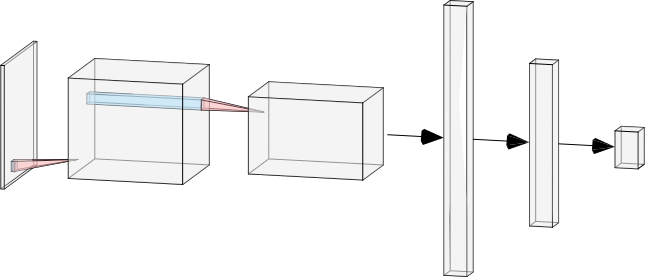
\includegraphics[width=.9\textwidth]{cnn.pdf}
        };

        \node at (1,-0.5) {Convolution};
        \node at (5,-0.5) {Convolution};
        \node at (9.5,-0.5) {Flatten};
        \node at (11.8,-0.5) {Dense};
        \node at (14,-0.5) {Dense};

        \node at (0.3,7) {$40\times40\times1$};
        \node at (3.3,7) {$20\times20\times32$};
        \node at (7.4,7) {$10\times10\times32$};
        \node at (10.8,7) {$3200$};
        \node at (12.8,7) {$128$};
        \node at (14.9,7) {$3$};
    \end{tikzpicture}
    \caption{Structure of the CNN (Graphic created using NN-SVG \cite{LeNail2019NN})}
    \label{fig:det:cnnStructure}
\end{figure}

The training data consists of $2,406$ hand labeled patches extracted from point clouds of the \ac{d435}. To enlarge the dataset the training data has been augmented by factor ten, this is done by mirroring the image along the $y$-axis, rotating the point cloud up to $10^\circ$ around the axes and adding noise to the image. From the training data 10\% of the data is used for verification during training to detect overfitting.

The \ac{cnn} has been trained over $200,000$ epochs using the Adadelta optimizer with cross entropy used as the loss. The learning rate started at 0.002, after $25,000$ epochs the learning rate was set to 0.0005 and after $55,000$ epochs it was reduced to 0.0001. During training both the accuracy, that is the number of correctly labeled images divided by the total number of images, and the loss for both the training and the validation data have been calculated to track the performance of the
\ac{cnn}.

\subsection{Bounding Box Estimate} \label{sec:det:bbe}
For the later stages of planning it is of great importance to not only know the position of objects but additionally the dimension and orientation of the objects. 
Especially for obstacles and pedestrians it is important to estimate the size, as these objects need to be passed.
For signs the bounding box is used as a region of interest for the following classification.
As both obstacles and pedestrians are box shaped the shape of objects is estimated by fitting a bounding box to the cluster.
The objects are always placed flat on the ground, thus the roll and pitch angles are assumed to be zero. 

The bounding box estimation is done in three steps: first the heading (yaw) of the bounding box is estimated, in the second step the size of the bounding box in the $x$ and $y$ dimension is estimated and in the last step the size in the $z$ dimension is estimated.

The heading vector is calculated using the \ac{pca}, identical to \ref{sec:det:originalExtraction}.
Using the heading vector the horizontal vector that is orthogonal to the heading vector can be calculated:
\begin{equation}
    \vec{v}_\text{orth} =
        \normalize{
            \begin{pmatrix}
                0 \\ 0 \\ 1
            \end{pmatrix}
            \times \vec{v}_\text{heading}
        }
\end{equation}

A point can now be transformed into the rotated coordinate system:
\begin{equation}
    \vec{p}_\text{transformed} =
        \begin{pmatrix}
            & \vec{v}_\text{heading} & \\ & \vec{v}_\text{orth} & \\ 0 & 0 & 1
        \end{pmatrix}
        \cdot \left( \vec{p} - \vec{p}_\text{mean} \right)
\end{equation}

By transforming all points of a cluster $c$ a transformed cluster $\tilde{c}$ can be calculated.
Using the transformed points the respective minimum and maximum values can be calculated similar to equation \ref{eqn:det:minx} to \ref{eqn:det:maxy}.
The maximum values can now be used to form the four corner points:
\begin{eqnarray}
    \vec{p}_{0,\text{transformed}} &=& 
        \begin{pmatrix}
            x_\text{min,transformed} \\ y_\text{min,transformed} \\ 0
        \end{pmatrix} \\
    \vec{p}_{1,\text{transformed}} &=& 
        \begin{pmatrix}
            x_\text{min,transformed} \\ y_\text{max,transformed} \\ 0
        \end{pmatrix} \\
    \vec{p}_{2,\text{transformed}} &=& 
        \begin{pmatrix}
            x_\text{max,transformed} \\ y_\text{max,transformed} \\ 0
        \end{pmatrix} \\
    \vec{p}_{3,\text{transformed}} &=& 
        \begin{pmatrix}
            x_\text{max,transformed} \\ y_\text{min,transformed} \\ 0
        \end{pmatrix}
\end{eqnarray}
This guarantees, that all points are inside of the bounding box.

By transforming the corner points back into the original coordinate system the bounding box can be calculated:
\begin{equation}
    \vec{p} = {
        \begin{pmatrix}
            & \vec{v}_\text{heading} & \\ & \vec{v}_\text{orth} & \\ 0 & 0 & 1
        \end{pmatrix}
    }^{-1} \cdot \vec{p}_\text{transformed} + \vec{p}_\text{mean}
\end{equation}

For the dimensions of the bounding box along the $z$-Axis the minimum and maximum values are calculated identical to equation \ref{eqn:det:minz} and \ref{eqn:det:maxz}. These two values are selected as the height of the bottom and top of the bounding box.

\subsection{Ground Estimate}
For the detection of the slope the ground plane is approximated by a single plane. 
At the beginning of a slope the ground consists of two slopes, thus the single plane is not able to perfectly fit the ground. As the ground estimate is only used as a binary detector for the slope, the angle of the slope is not important, this accuracy is still sufficient.

To fit the plane all cells labeled as ground are taken into account. For each cell a single point is determined by the centre of the cell and the average $z$ values of all points in the cell. In contrast to using all points which are part of a ground cell this approach is not influenced by the varying density of the point cloud. Thus the plane is not biased towards the ground points closer to the vehicle.

The plane is chosen such that, the average squared error between the points and the plane is minimal. The algorithm used for this least squares approach is the algorithm presented in Section \ref{sec:theo:leastSquaresPlane}.
